\documentclass[twoside,english]{uiofysmaster}

%\bibliography{references}

\author{Fredrik Wilhelm Holmen}
\title{Master thesis Wilhelm Coupled Cluster}
\date{Autumn 2015}

\begin{document}
% set space around equations
\setlength{\belowdisplayskip}{12pt} \setlength{\belowdisplayshortskip}{12pt}
\setlength{\abovedisplayskip}{12pt} \setlength{\abovedisplayshortskip}{12pt}


\maketitle

\begin{abstract}
  This is an abstract text.
\end{abstract}

\begin{dedication}
  To someone
  \\\vspace{12pt}
  This is a dedication to my cat.
\end{dedication}

\begin{acknowledgements}
  I acknowledge my acknowledgements.
\end{acknowledgements}

\tableofcontents



\begin{chapter}{Introduction}
  This is a very nice introduction to my myster thesis.
  or ..
  lol
\end{chapter}





\begin{chapter}{Quantum Mechanics}
 
 \begin{section}{Postulates}
 	
 \end{section}

 \begin{section}{Hermitian Operators}
 	
 \end{section}

 \begin{section}{Pauli's Exclusion Principle}
 	
 \end{section}

	\begin{section}{The Variational Principle}

	\end{section}

	\begin{section}{Slater Determinant}
		A system composed of a nuclei and electrons moving in accordance to the forces of electromagnetic attraction can be described by assigning each electron
		a wave function 
		\begin{align}
			\phi_i(\mathbf{x}_i)
		\end{align}
		Where $\mathbf{x}_i$ is the position vector for the electron i. Describing a system of many electrons can be done writing a Slater Determinant
		\begin{align}
			\ket{\Phi_0} = \frac{1}{ \sqrt{N!} } \left|\begin{matrix}
				\phi_1(\mathbf{x}_1) & \phi_2(\mathbf{x}_1) & ... & \phi_N(\mathbf{x}_1) \\
				\phi_1(\mathbf{x}_2) & \phi_2(\mathbf{x}_2) & ... & \phi_N(\mathbf{x}_2) \\
				... & & & \\
				\phi_1(\mathbf{x}_N) & \phi_2(\mathbf{x}_N) & ... & \phi_N(\mathbf{x}_N) 
			\end{matrix} \right|
		\end{align}
		This way of writing the many-body wave function will represent linear a combination of products of the one-body wave functions $\phi_i$'s and all the electronic coordinates
		$\mathbf{x}_i$ distributed among them in all possible ways. Exchanging two lines will change the sign such that the Slater Determinant will respect the anti-symmetry 
		requirement. \par
		We can choose the one-body wave functions that is most rewarding the specified system. When calculating on electrons moving with respect to a nuclei, one can choose the wave
		functions to be the 1s, 2s, 2p, .. orbitals. This representation will not, however, take into account the Colombic repulsion between two electrons and will only be an 
		approximation to the true wavefunction, $\ket{\Psi}$.
	\end{section}

\end{chapter}





\begin{chapter}{Second Quantization}
 Second quantization is a new method of representing states and operators. 
 \begin{section}{Annihilation and Creation operators}
 	We introduce a new way of writing states using the mathematical technique known as second quantization. The main goal is to treat states without paying attention
  	to individual particle coordinates. We represent the empty space with the symbol for vacuum
  	\begin{align}
  		\ket{0}
  	\end{align}
  	To represent a state, we use a creation operator to add the state to the vacuum.
  	\begin{align}
  		\hat a_i^{\dagger} \ket{0} = \ket{\phi_i}
  	\end{align}
  	And the annihilation operator will remove the particle again. 
  	\begin{align}
  		\hat a_i \ket{\phi_i} = \ket{0}
  	\end{align}
  	Trying to add a new particle to an already filled state and removing an unoccupied state results in zero.
  	\begin{align}
  		\hat a_i^{\dagger} \ket{\phi_i} = 0 \;\;\;\;\; \hat a_i \ket{0} = 0
  	\end{align}
  	We can now write the Slater determinant as a chain of creation operators
  	\begin{align}
  		\hat a_1^{\dagger} \hat a_2^{\dagger}... \hat a_N^{\dagger} \ket{0}
  	\end{align}
  	Permutations of the operators introduces a sign-change, which is equivalent to interchanging rows in the determinant. This 
  	\begin{align}
  		\hat a_1^{\dagger} \hat a_2^{\dagger} \ket{0} = \ket{\phi_1 \phi_2} = -\ket{\phi_2 \phi_1} = -\hat a_2^{\dagger} \hat a_1^{\dagger} \ket{0}
  	\end{align}
  	So we can see that the second quantization respects the antisymmetrization condition. Thus, these operators follow the anti commutation relations
  	\begin{align}
  		\{ \hat a_i^{\dagger} \hat a_j \} = \delta_{ij} \;\;\;\;\; \{ \hat a^{\dagger}_i \hat a^{\dagger}_j \} = 0 \;\;\;\;\; \{ \hat a_i \hat a_j \} = 0
  	\end{align}
  	Where $\delta_{ij}$ is the Kronecher delta. 
 \end{section}

 \begin{section}{Representation of Operators}
 	
 \end{section}

 \begin{section}{Fermi Vacuum}
 	
 \end{section}

 \begin{section}{Normal Ordering and Wick's Theorem}
 	
 \end{section}

 \begin{section}{Partitioning the Hamiltonian}
 	
 \end{section}
 
\end{chapter}




\begin{chapter}{Many-Body Methods}
	We have already justified the use of a Slater Determinant to describe the first approximation of the full wave function, $\ket{\Psi}$. Where
	\begin{align}
		\ket{\Psi} \approx \ket{\Phi_0} = 	\frac{1}{ \sqrt{N!} } \left|\begin{matrix}
			\phi_1(\mathbf{x}_1) & \phi_2(\mathbf{x}_1) & ... & \phi_N(\mathbf{x}_1) \\
			\phi_1(\mathbf{x}_2) & \phi_2(\mathbf{x}_2) & ... & \phi_N(\mathbf{x}_2) \\
			... & & & \\
			\phi_1(\mathbf{x}_N) & \phi_2(\mathbf{x}_N) & ... & \phi_N(\mathbf{x}_N) 
		\end{matrix} \right|
	\end{align}	
	This first representation fails to account for the Coulombic interrraction between the electrons, and we need higher-order approximations on top 
	of the Slater Determinant to improve our results. \par
	This chapter will look at three methods, namely the Configuration interraction, Many-body Perturbation theory and Hartree-Fock approximations. The
	Master thesis is on Coupled Cluster theory, and that will be more elaborately explained in it's own chapter. It is useful to benchmark Coupled Cluster 
	with similar many-body method. 

 \begin{section}{Configuration Interraction}
 		We can write the configuration interaction wavefunction as 
  	\begin{align}
  		\ket{\Psi_{CI}} = (1 + \hat C) \ket{\Phi_0} 
   	\end{align}
  	\begin{align}
  		\hat C = \hat C_1 + \hat C_2 + ... =  \sum_{ia} c_i^a a_a^{\dagger} a_i + \frac{1}{4} \sum_{ijab} c_{ij}^{ab} a_a^{\dagger} a_b^{\dagger} a_j a_i + ...
   	\end{align}
 \end{section}	

 \begin{section}{Many-body Perturbation Theory}
 	
 \end{section}

 \begin{section}{Hartree-Fock approximations}
 	
 \end{section}

\end{chapter}




\begin{chapter}{Coupled-Cluster Theory}
 	In Coupled Cluster theory, the ansatz we make is to make an expansion in the wave function
 	\begin{align}
 		\ket{\Psi} \approx e^{\hat T} \ket{\Psi_0}
  	\end{align}
  	The operator $\hat T$ is a linear combination of the cluster operators
  	\begin{align}
  		\hat T = \hat T_1 + \hat T_2 + \hat T_3 + ... + \hat T_N
  	\end{align}
  	Where the operators represent
  	\begin{align}
  		T_1 &= \sum_{ia} t_i^a \hat a_a^{\dagger} \hat a_i \\
  		T_2 &= \frac{1}{2} \sum_{ijab} t_{ij}^{ab} \hat a_a^{\dagger}\hat a_b^{\dagger} \hat a_j \hat a_i \\
  		T_2 &= \left(\frac{1}{n!}\right)^2 \sum_{ij..ab..}^n t_{ij..n}^{ab..n} \hat a_a^{\dagger}\hat a_b^{\dagger} ...\hat a_n^{\dagger} \hat a_n ... \hat a_j \hat a_i \\
  	\end{align}

  	We can write the configuration interaction wavefunction as 
  	\begin{align}
  		\ket{\Psi_{CI}} = (1 + \hat C) \ket{\Phi_0} 
   	\end{align}
  	\begin{align}
  		\hat C = \hat C_1 + \hat C_2 + ... =  \sum_{ia} c_i^a a_a^{\dagger} a_i + \frac{1}{4} \sum_{ijab} c_{ij}^{ab} a_a^{\dagger} a_b^{\dagger} a_j a_i + ...
   	\end{align}
   	Comparing this linear expansion to the exponential expansion from Coupled Cluster, we can see that
   	\begin{align}
   		\hat C_2 = \hat T_2 + \frac{1}{2} T_1^2
   	\end{align}
   	Where we can see that even if we truncate Configuration Interaction and Coupled Cluster at the same level, there are more \textit{disconnected} wave function contributions (REFERENCE page 17 IN C\&S) in the Coupled Cluster theory. Both the Coupled Cluster and Configuration Interaction theory provides the exact energy by including the operators to infinite order, i.e. no truncation. 

  	\begin{section}{Size Extensivity}
  		It can be important to have a wave function that scales with size. Imagine a two particles, $X$ and $Y$ with infinity separation, they do not interact. This means we should be able to write the total energy as
  		\begin{align}
  			E = E_X + E_Y
  		\end{align}
  		Doing Coupled Cluster
  		\begin{align}
  			\hat T = \hat T_X + \hat T_Y 
  		\end{align}
  		\begin{align}
  			\ket{\Psi}_{CC} = e^{\hat T_X + \hat T_Y} \ket{\Phi_0} = e^{\hat T_X} e^{\hat T_Y} \ket{\Psi_0}
  		\end{align}
  		Since we can write the reference state as a product of the two seperated parts, we are able to write
  		\begin{align}
  			E_{CC} = E_{CC}^X + E_{CC}^Y
  		\end{align}
  		This means Coupled Cluster is size extensive, contrary to the Configuration Interaction. 
  	\end{section}

  	\begin{section}{The CCD Equations}
  		The Coupled Cluster Doubles equations can be finalized as
  		\begin{align}
  			E_{CCD} = E_{ref} + \Delta E_{CCD} 
  		\end{align}
  		With the reference energy defined as 
  		\begin{align}
  			E_{ref} = \sum_i \left< i \middle| \hat h_0 \middle| j\right> + \sum_{ij} \left<ij\middle|\hat v\middle|ij\right> + \frac{1}{2}Av_0
  		\end{align}
  		and the corrolation energy given by
  		\begin{align}
  			\Delta E_{CCD} = \frac{1}{4} \sum_{ijab}\left<ij\middle|\hat v\middle|ab\right> t_{ij}^{ab}
  		\end{align}
  		$v_0$ is a constant, nonzero for the finite electron gas. After several applications of Wick's theorem, the amplitude equations can be reduced to
  		\begin{align}
  			(\epsilon_i + \epsilon_j - \epsilon_a - \epsilon_b) t_{ij}^{ab} = \left<ab\middle|\hat v\middle|ij\right> + \frac{1}{2} \sum_{cd}\left<ab\middle|\hat v\middle|cd\right>t_{ij}^{cd} \\
  			+ \frac{1}{2} \sum_{kl} \left<kl\middle|\hat v\middle|ij\right>t_{kl}^{ab} + \hat P\left(ij\middle|ab\right) \sum_{kc}\left<kb\middle|\hat v\middle|cj\right>t_{ik}^{ac} \\
  			+ \frac{1}{4} \sum_{klcd}\left<kl\middle|\hat v\middle|cd\right>t_{ij}^{cd} t_{kl}^{ab} + \frac{1}{2} \hat P\left(ij\middle|ab\right) \sum_{klcd}\left<kl\middle|\hat v\middle|cd\right>t_{ik}^{ac} t_{lj}^{db}\\
  			- \frac{1}{2}\hat P(ij) \sum_{klcd}\left<kl\middle|\hat v\middle|cd\right>t_{ik}^{ab} t_{jl}^{cd} - \frac{1}{2}\hat P(ab) \sum_{klcd}\left<kl\middle|\hat v\middle|cd\right>t_{kl}^{bd} t_{ij}^{ac}
  			\label{CCD_equations1}
  		\end{align}
  		Where we have defined
  		\begin{align}
  			\hat P(ij) = 1 - \hat P_{ij}
  		\end{align}
  		Where $\hat P_{ij}$ interchanges the two particles occupying the quantum states $i$ and $j$. Furthermore, we define the operator 
  		\begin{align}
  			\hat P\left( ij \middle| ab \right) = (1 - \hat P_{ij}) (1 - \hat P_{ab})
  		\end{align}
  		We notice that some parts are linear in the amplitude, while some are quadradic. Sorting them into the linear and quadradic parts, $L$ and $Q$ respectably, I get
  		\begin{align}
  			L(t_{ij}^{ab}) = \frac{1}{2} \sum_{cd}\left<ab\middle|\hat v\middle|cd\right>t_{ij}^{cd} + \frac{1}{2} \sum_{kl} \left<kl\middle|\hat v\middle|ij\right>t_{kl}^{ab} + \hat P\left(ij\middle|ab\right) \sum_{kc}\left<kb\middle|\hat v\middle|cj\right>t_{ik}^{ac}
  		\end{align}
  		and 
  		\begin{align}
  			Q(t_{ij}^{ab}t_{ij}^{ab}) = \frac{1}{4} \sum_{klcd}\left<kl\middle|\hat v\middle|cd\right>t_{ij}^{cd} t_{kl}^{ab} + \frac{1}{2} \hat P\left(ij\middle|ab\right) \sum_{klcd}\left<kl\middle|\hat v\middle|cd\right>t_{ik}^{ac} t_{lj}^{db} \\
  			- \frac{1}{2}\hat P(ij) \sum_{klcd}\left<kl\middle|\hat v\middle|cd\right>t_{ik}^{ab} t_{jl}^{cd} - \frac{1}{2}\hat P(ab) \sum_{klcd}\left<kl\middle|\hat v\middle|cd\right>t_{kl}^{bd} t_{ij}^{ac}
  		\end{align}
  		Labeling each term for practical reasons	
  		\begin{align}
  			L_a &= \frac{1}{2} \sum_{cd}\left<ab\middle|\hat v\middle|cd\right>t_{ij}^{cd} \\
  			L_b &= \frac{1}{2} \sum_{kl} \left<kl\middle|\hat v\middle|ij\right>t_{kl}^{ab} \\
  			L_c &= \hat P\left(ij\middle|ab\right) \sum_{kc}\left<kb\middle|\hat v\middle|cj\right>t_{ik}^{ac} \\
  			Q_a &= \frac{1}{4} \sum_{klcd}\left<kl\middle|\hat v\middle|cd\right>t_{ij}^{cd} t_{kl}^{ab} \\
  			Q_b &= \frac{1}{2} \hat P\left(ij\middle|ab\right) \sum_{klcd}\left<kl\middle|\hat v\middle|cd\right>t_{ik}^{ac} t_{lj}^{db} \\
  			Q_c &= - \frac{1}{2}\hat P(ij) \sum_{klcd}\left<kl\middle|\hat v\middle|cd\right>t_{ik}^{ab} t_{jl}^{cd} \\
  			Q_d &= - \frac{1}{2}\hat P(ab) \sum_{klcd}\left<kl\middle|\hat v\middle|cd\right>t_{kl}^{bd} t_{ij}^{ac}
  		\end{align}
   	\end{section}

  	\begin{section}{Intermediates}
  		As Coupled Cluster computations are consume large amounts of computational power, researchers are spending much effort trying to reduce computational cost. One way of reducing the cost is by refactoring the amplitude equations such that we can perform an intermediate computation first and use the result to compute various diagrams later. 

  		Rewriting the equation, (\ref{CCD_equations1}) for CCD amplitudes (Source: Gustav Baardsen / Audun):
  		\begin{align}
  			(\epsilon_i + \epsilon_j - \epsilon_a - \epsilon_b) t_{ij}^{ab} = \left<ab\middle|\hat v\middle|ij\right> + \frac{1}{2} \sum_{cd}\left<ab\middle|\hat v\middle|cd\right>t_{ij}^{cd} \\
  			+ \frac{1}{2} \sum_{kl} t_{kl}^{ab} \left[ \left<kl\middle|\hat v\middle|ij\right> + \frac{1}{2} \sum_{cd} \left<kl\middle|\hat v\middle|cd\right> t_{ij}^{cd} \right] \\
  			+ \hat P\left(ij\middle|ab\right) \sum_{kc} t_{ik}^{ac} \left[ \left<kb\middle|\hat v\middle|cj\right> + \frac{1}{2}\sum_{ld}\left<kl\middle|\hat v\middle|cd\right>t_{lj}^{db} \right] \\
  			- \frac{1}{2} \hat P(ij) \sum_{k} t_{ik}^{ab} \left[ \sum_{lcd} \left<kl\middle|\hat v\middle|cd\right> t_{jl}^{cd} \right] \\
  			- \frac{1}{2} \hat P(ab) \sum_{c} t_{ij}^{ac} \left[ \sum_{kld} \left<kl\middle|\hat v\middle|cd\right> t_{kl}^{bd} \right]
  		\end{align}
  		We can now define, and precompute the following values
  		\begin{align}
  			I_1 = \left<kl\middle|\hat v\middle|ij\right> + \frac{1}{2} \sum_{cd} \left<kl\middle|\hat v\middle|cd\right> t_{ij}^{cd} \\
  			I_2 = \left<kb\middle|\hat v\middle|cj\right> + \frac{1}{2}\sum_{ld}\left<kl\middle|\hat v\middle|cd\right>t_{lj}^{db} \\
  			I_3 = \sum_{lcd} \left<kl\middle|\hat v\middle|cd\right> t_{jl}^{cd} \\
  			I_4 = \sum_{kld} \left<kl\middle|\hat v\middle|cd\right> t_{kl}^{bd}
  		\end{align}
  		We can now redefine the CCD equation 
  		\begin{align}
  			(\epsilon_i + \epsilon_j - \epsilon_a - \epsilon_b) t_{ij}^{ab} = \left<ab\middle|\hat v\middle|ij\right> + \frac{1}{2} \sum_{cd}\left<ab\middle|\hat v\middle|cd\right>t_{ij}^{cd} + \frac{1}{2} \sum_{kl} t_{kl}^{ab} I_1 \\
  			+ \hat P\left(ij\middle|ab\right) \sum_{kc} t_{ik}^{ac} I_2 - \frac{1}{2} \hat P(ij) \sum_{k} t_{ik}^{ab} I_3  - \frac{1}{2} \hat P(ab) \sum_{c} t_{ij}^{ac} I_4
  		\end{align}
  		Leading to a reduction of computational cost from $\mathcal{O}(h^4 p^4)$ to $\mathcal{O}(h^4 p^2)$


  	\end{section}

\end{chapter}




\begin{chapter}{The Pairing Model}
	The first system I look at is the pairing model. The pairing model has four energy levels with degeneracy two, one for positive and negative spins. I have 
	used a system consisting of four electrons filling up the four lower-most states up to the Fermi level. 
	\begin{figure}[h]
		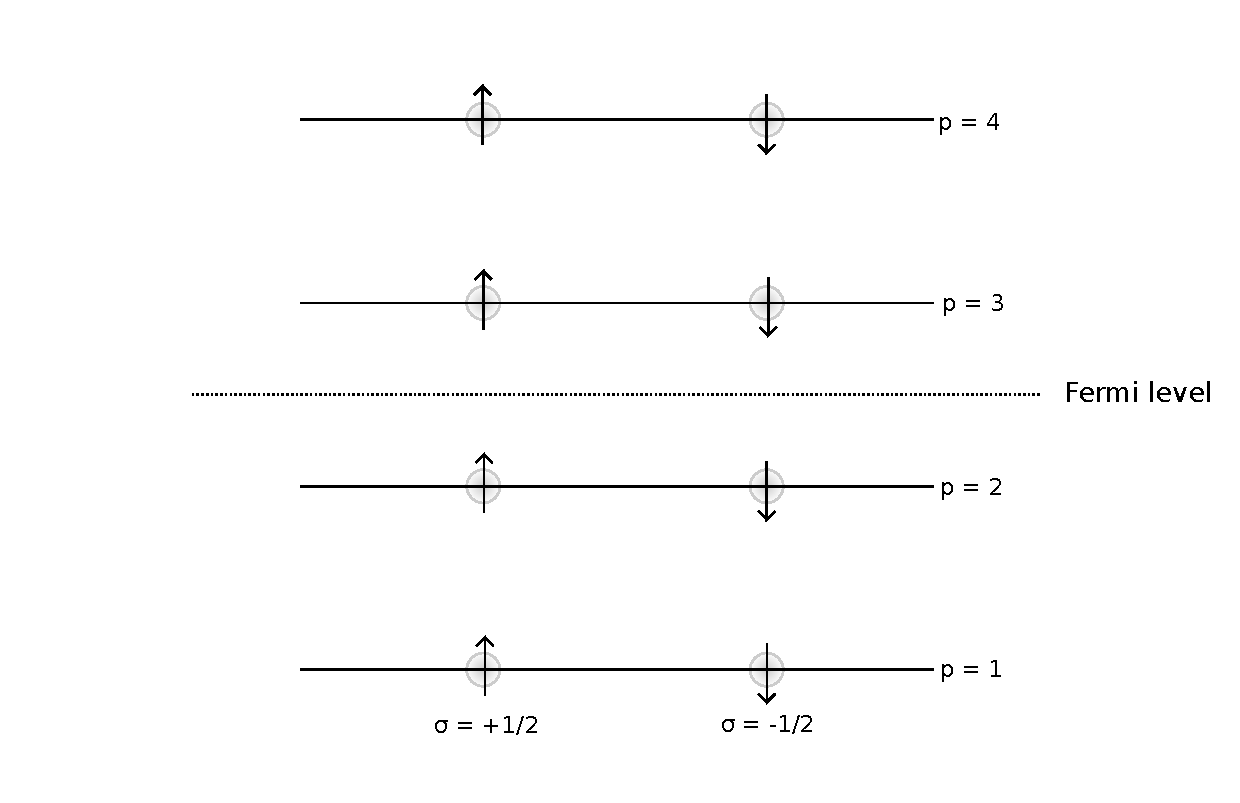
\includegraphics[width=\textwidth]{Figures/Pairing_model.pdf}
		\label{PairingModel_1}
		\caption{A figure depicting a 4 particles-4 holes state. The system consists of occupied particle states below the Fermi level and unoccupied hole states above Fermi level.}
	\end{figure}
	
	\begin{section}{The Hamiltonian}
		We limit ourselves to a two-body interaction, writing the Hamiltonian as
		\begin{align}
			\hat H = \sum_{\alpha \beta} \left< \alpha \right| \hat h_0 \left| \beta \right> \hat a_{\alpha}^{\dagger} \hat a_{\beta} 
			        + \frac{1}{4} \sum_{\alpha \beta \gamma \delta} \left< \alpha \beta \middle| \hat v_0 \middle| \gamma \delta \right> \hat a_{\alpha}^{\dagger} \hat a_{\beta}^{\dagger} \hat a_{\delta} \hat a_{\gamma}
		\end{align}
		We use the complete basis $\left| \alpha \right>$ and define the set as eigenvalues of the one-body operator, $\hat h_0$. 
		
		The system does require that the total spin is equal to $0$. In addition we will not allow spin pairs to be broken, i.e.\  singly excitated states are not allowed. 
		\begin{align}
			\left| \Psi_i^a \right> = 0 
		\end{align}	
		We introduce the double creation and annihilation operator. 
		\begin{align}
			\hat P_{pq}^{\dagger} = \hat a_{p \sigma}^{\dagger} \hat a_{p -\sigma}^{\dagger}
		\end{align}
		\begin{align}
			\hat P_{pq} =  a_{q \sigma} a_{q -\sigma}
		\end{align}

		We can rewrite the Hamiltonian as an unperterturbed part and a perturbation
		\begin{align}
			\hat H = \hat H_0 + \hat V
		\end{align}
		\begin{align}
			\hat H_0 = \xi \sum_{p \sigma} (p-1) \hat a_{p \sigma}^{\dagger} \hat a_{p \sigma}
		\end{align}
		\begin{align}
			\hat V = - \frac{1}{2}g \sum_{pq} \hat a_{p +}^{\dagger} \hat a_{p-}^{\dagger} \hat a_{q-} \hat a_{q+}
		\end{align}
		The value of $\xi$ determines the spacing between the energy levels, which I have set to $1$. This will not impact the insight attained solving this system. $p$ and $q$ determines the energy level. $\sigma$ is the spin, with value either $+\frac{1}{2}$ or $-\frac{1}{2}$. Both the unperturbed and perturbed Hamiltonian keeps total spin at $0$

		We can normal order the Hamiltonian by Wicks general theorem. 
		\begin{align}
			a_p^{\dagger} a_q = \left\{ a_p^{\dagger}a_q \right\} + \delta_{pq \in i}
		\end{align}
		\begin{align}
			a_p^{\dagger} a_q^{\dagger} a_s a_r = \left\{ a_p^{\dagger}a_q^{\dagger} a_s a_r \right\} +\left\{a_p^{\dagger}a_r\right\} \delta_{qs\in i} - \left\{a_p^{\dagger}a_s\right\} \delta_{qr\in i} \\
			+\left\{a_q^{\dagger}a_s\right\} \delta_{pr\in i} \
			- \left\{a_q^{\dagger}a_r\right\} \delta_{ps\in i} + \delta_{pr \in i} \delta_{qs \in i} - \delta_{ps \in i}\delta_{qr \in i}
		\end{align}
		Which gives the Normal-ordered Hamiltonian
		\begin{align}
			\hat H = \hat H_N + E_{ref}
		\end{align}
		\begin{align}
			\hat H_N = \hat F_N + \hat W 
		\end{align}
		\begin{align}
			\hat F_N =  \sum_{pq} h_{pq} \left\{ \hat a_{p \sigma}^{\dagger} \hat a_{p \sigma} \right\}
			- \sum_{pqi} \left< pi || qi \right> \left\{ \hat a_{p +}^{\dagger} \hat a_{q -} \right\}
		\end{align}
		\begin{align}
			\hat W = - \frac{1}{2} \sum_{pqrs} \left< pq || rs \right> \left\{ \hat a_{p +}^{\dagger} \hat a_{p-}^{\dagger} \hat a_{q-} \hat a_{q+} \right\}
		\end{align}
		\begin{align}
 			E_{ref} = \sum_{i} h_{ii} + \frac{1}{2} \sum_{ij} \left< ij \middle| \middle| ij \right>
		\end{align}

	\end{section}


	\begin{section}{Configuration Interaction theory}
		This system is a good way to benchmark various methods as we can compute the exact solution using Full Configuration Interaction. 

		\begin{figure}[h]
			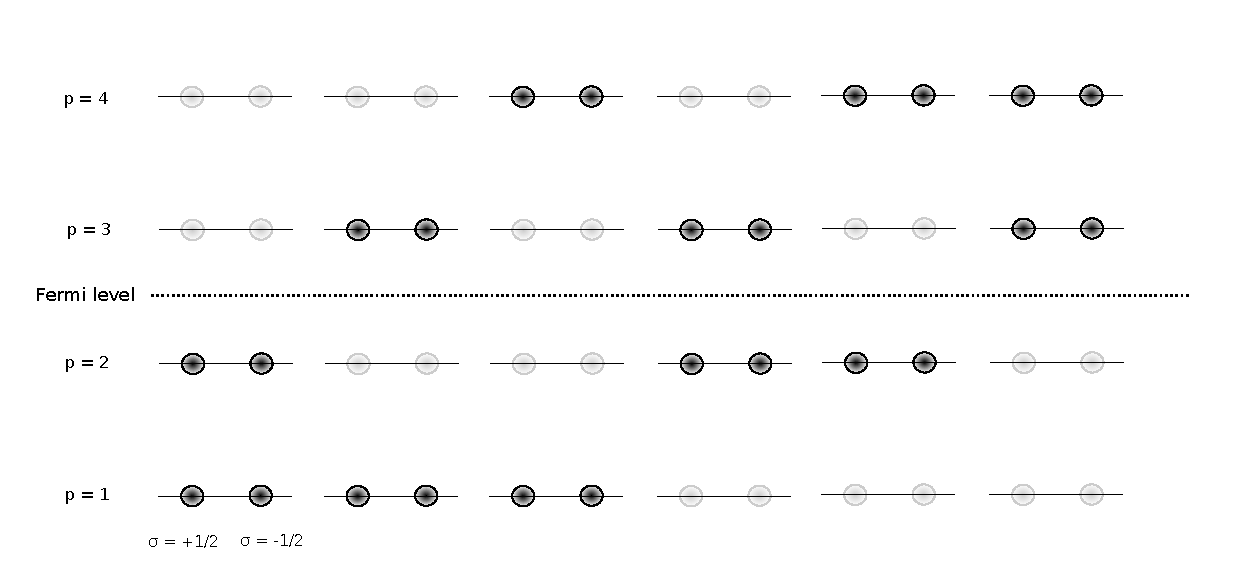
\includegraphics[width=1.1\linewidth]{Figures/Pairing_model2.pdf}
			\label{PairingModel_2}
			\caption{Configuration space for given pairing model showing all possible distributions of electrons}
		\end{figure}

 	We need to diagonalize the Hamiltonian matrix looking at the linear combination of all different compinations of 
	\begin{align}
		\hat{ \mathcal{H} } = \left(  \begin{matrix}
			& \left| \Phi_0 \right> & \left| \Phi_{12}^{56} \right> & \left| \Phi_{12}^{78} \right> & \left| \Phi_{34}^{56} \right> & \left| \Phi_{34}^{78} \right> & \left| \Phi_{1234}^{5678} \right> \\ 
			\left< \Phi_0 \right| &   &   &   &   &   & \\
			\left< \Phi_{12}^{56} \right| &   &   &   &   &   & \\
			\left< \Phi_{12}^{78} \right| &   &   &   &   &   & \\
			\left< \Phi_{34}^{56} \right| &   &   &   &   &   & \\
			\left< \Phi_{34}^{78} \right| &   &   &   &   &   & \\
			\left< \Phi_{1234}^{5678} \right| &   &   &   &   &   & 
		\end{matrix} \right)
	\end{align}

 Excluding the 4p-4h excitations one does not diagonalize the exact matrix, but rather the approximated matrix known from Configuration Interaction. 

 The diagonal elements are calculated using Wick's theorem. Looking first at the ground state calculation with the unperturbed Hamiltonian part
 \begin{align}
 	\left< \Phi_0 \middle| \hat{\mathbf{H_0}} \middle| \Phi_0 \right> 
 \end{align}
 \begin{align}
 	\left< \right|  a_{2 \downarrow}  a_{2 \uparrow} a_{1 \downarrow} a_{1 \uparrow} \sum_{p \sigma} \delta (p-1) a_{p \sigma}^{\dagger} a_{p \sigma} 
 	a_{1 \uparrow}^{\dagger} a_{1 \downarrow}^{\dagger} a_{2 \uparrow}^{\dagger} a_{2 \downarrow}^{\dagger} \left| \right> 
 \end{align}
 Which we see can contract in four different ways, resulting in 
 \begin{align}
 	2 \delta (1-1) + 2 \delta (2-1) = 2 \delta
 \end{align}

 And the perturbation part
 \begin{align}
 	\left< \Phi_0 \middle| \hat{\mathbf{V}} \middle| \Phi_0 \right>
 \end{align}
 \begin{align}
 	\left< \right| a_{2 \downarrow}  a_{2 \uparrow} a_{1 \downarrow} a_{1 \uparrow} \left( -g / 2 \sum_{pq} a_{p \uparrow}^{\dagger} a_{q \downarrow}^{\dagger} a_{q \downarrow} a_{p \uparrow} \right) 
 	a_{1 \uparrow}^{\dagger} a_{1 \downarrow}^{\dagger} a_{2 \uparrow}^{\dagger} a_{2 \downarrow}^{\dagger} \left| \right> 
 \end{align}
 As we can see, there are two ways this can contract, each contributing with the constant factor, $-g / 2$
 Resulting in the final Hamiltonian matrix 
 \begin{align}
 	\hat{\mathcal{H}} = \left( \begin{matrix}
 		2 \delta - g & -g / 2 & -g / 2 & -g / 2 & -g / 2 & 0  \\
 		-g / 2 & 4 \delta - g & -g / 2 & -g / 2 & 0 & -g / 2  \\
 		-g / 2 & -g / 2 & 6 \delta - g & 0 & -g / 2 & -g / 2 \\
 		-g / 2 & -g / 2 & 0 & 6 \delta - g & -g / 2 & -g / 2 \\
 		-g / 2 & 0 & -g / 2 & -g / 2 & 8 \delta - g & -g / 2 \\
 		0 & -g / 2 & -g / 2 & -g / 2 & -g / 2 & 10 \delta - g 
 	\end{matrix} \right)
 \end{align}

 \end{section}

 \begin{section}{Diagrammatic Rules}
 	One can visualize many-body quantum physics by using diagrams. 

 	
 \end{section}

 \begin{section}{Many-Body Perturbation Theory}
 	The Perturbation theory presents a non-iterative approach to approximating the ground state energy. The approach is similar to previous methods. We start by splitting the Hamiltonian into a solvable part and a perturbation. 
 	\begin{align}
 		\hat H = \hat H_0 + \hat V
 	\end{align}
 	Where we have chosen our basis such that
 	\begin{align}
 		\hat H_0 \left| \Psi_0 \right>  = W_0 \left| \Psi_0 \right>
 	\end{align}
 	We split the basis aswell
 	\begin{align}
 		\left| \Psi_0 \right> = \left| \Phi_0 \right> + \sum_i^{\infty} c_i \left| \phi_i \right>
 	\end{align}
 	Assuming intermediate normalization
 	\begin{align}
 		\left< \Phi_0 | \Psi_0 \right> = 1
 	\end{align}
	We can calculate the total exact energy
 	\begin{align}
 		E = \left< \Phi_0 \right| \hat H_0 \left| \Psi_0 \right> + \left< \Phi_0 \right| \hat V \left| \Psi_0 \right>
 	\end{align}
 	Where we know that
 	\begin{align}
 		 \left< \Phi_0 \right| \hat H_0 \left| \Psi_0 \right>  = W_0
 	\end{align}
 	And we get the corrolation energy
 	\begin{align}
 		E - W_0 = \Delta E = \left< \Phi_0 \right| \hat V \left| \Psi_0 \right>
 	\end{align}
 	We will usually aim to compute this energy when doing MBPT. 

 	\begin{subsection}{General derivation of Many Body Particle Theory equations}
 		Looking at the equation
 		\begin{align}
 			\hat V \left| \Psi_0 \right> = \hat H \left| \Psi_0 \right> + \hat H_0 \left| \Psi_0 \right> 
 		\end{align}
 		We reorganize and add the term $\omega \left| \Psi_0 \right>$ on both sides
 		\begin{align}
 			\hat V \left| \Psi_0 \right> + \omega \left| \Psi_0 \right> - \hat H \left| \Psi_0 \right> = \omega \left| \Psi_0 \right> - \hat H_0 \left| \Psi_0 \right> 
 		\end{align}
 		Remembering that $\hat H \left| \Psi_0 \right> = E\left| \Psi_0 \right> $, we get 
 		\begin{align}
 			\left| \Psi_0 \right> = \frac{ \hat V + \omega - E }{\omega - \hat H_0} \left| \Psi_0 \right>
 			\label{pert_1}
 		\end{align}
 		Before continuing, we introduce the operators $\hat P$ and $\hat Q$, such that
 		\begin{align}
 			\left| \Psi_0 \right> = \hat P \left| \Psi_0 \right> + \hat Q \left| \Psi_0 \right> 
 			&= \left| \Phi_0 \right> \left< \Phi_0 \middle| \Psi_0 \right> + \sum_i \left| \Phi_i \right> \left< \Phi_i \middle| \Psi_0 \right> 
 			\label{pert_2} \\
 			&= \left| \Phi_0 \right> + \chi
 		\end{align}
 		Giving
 		\begin{align}
 			\left| \Phi_0 \right> = \hat P \left| \Psi_0 \right> \;\;\;\; \chi = \hat Q \left| \Psi_0 \right> 
 			\label{pert_3}
 		\end{align}
 		Using $\hat R(\omega) = \frac{\hat{Q}}{\left( \omega - \hat H_0 \right)}$ and multiplying both sides with $\hat Q$ from the left in equation (\ref{pert_1}) we attain
 		\begin{align}
 			\hat Q \left| \Psi_0 \right> = \hat R(\omega) \left( \hat V + \omega - E \right) \left| \Psi_0 \right>
 		\end{align}
 		Using equations (\ref{pert_2}) and (\ref{pert_3}), we get
 		\begin{align}
 			\left| \Psi_0 \right> = \left| \Phi_0 \right> + \hat R(\omega) \left( \hat V + \omega - E \right) \left| \Psi_0 \right>
 		\end{align}
 		This is an iterative scheme. We can substitute $\left| \Psi_0 \right>$ on the right hand side with the entire right hand side. This results in an infinite sum provided the series converges
 		\begin{align}
 			\left| \Psi_0 \right> = \sum_0^\infty \left\{ \hat R(\omega) (\hat V + \omega - E) \right\}^m \left| \Phi_0 \right>
 		\end{align}
 		The right hand side does include the energy, $E$, which must be computed using $ E = W_0 + \Delta E$, and
 		\begin{align}
 			\Delta E = \left< \Phi_0 \right| \hat V \left| \Psi_0 \right> 
 			= \sum_0^\infty \left< \Phi_0 \right| \hat V \left[ \hat R(\omega) (\hat V - E + \omega) \right]^m \left| \Phi_0 \right>  
 		\end{align}
 	\end{subsection}

 	\begin{subsection}{Equations for Reileigh-Schrodinger Perturbation Theory}
 		We can interpret $\omega$ different ways. I here present the Reileigh-Schrodinger Perturbation Theory which postulates that
 		\begin{align}
 			\omega = W_0 
 		\end{align}
 		Such that 
 		\begin{align}
 			\left| \Psi_0 \right> = \frac{ \hat V - \Delta E }{\omega - \hat H_0} \left| \Psi_0 \right>
 		\end{align}
 		and we get the final equations
 		\begin{align}
 			\left| \Psi_0 \right> = \sum_0^\infty \left\{ \hat R(\omega) (\hat V + - \Delta E) \right\}^m \left| \Phi_0 \right>
 		\end{align}
 		and
 		\begin{align}
 			\Delta E = \sum_0^\infty \left< \Phi_0 \right| \hat V \left[ \hat R(\omega) (\hat V - \Delta E) \right]^m \left| \Phi_0 \right>  
 		\end{align}
 		Taking a closer look at the energy-equations, we find that we can write the first orders as
 		\begin{align*}
 			E^{(1)} &= \left< \Phi_0 \right| \hat V \left| \Phi_0 \right>  = V_{00}\\
 			E^{(2)} &= \left< \Phi_0 \right| \hat V \hat R_0 \hat V \left| \Phi_0 \right> \\
 			E^{(3)} &= \left< \Phi_0 \right| \hat V \hat R_0 (\hat V - E^{(1)})  \hat R_0 \hat V \left| \Phi_0 \right> \\
 			E^{(4)} &= \left< \Phi_0 \right| \hat V \hat R_0 (\hat V - E^{(1)})  \hat R_0 (\hat V - E^{(1)}) \hat R_0 \hat V \left| \Phi_0 \right> 
 					- E^{(2)} \left< \Phi_0 \right| \hat V \hat R_0^2 \hat V \left| \Phi_0 \right>\\
  		\end{align*}
  		Because of the frequent appearance, we can rewrite $\hat V - E^{(1)}$ as
  		\begin{align}
  			\hat \Omega = \hat V - E^{(1)}
  		\end{align}
  		We name this new variable the wave operator
 	\end{subsection}

 	\begin{subsection}{Canonical Hartree-Fock}
 		In the pairing model, we work with the Normal-ordered Hamiltonian
 		\begin{align}
 			\hat H_N = \hat F_N^d + \hat F_N^0 + \hat W		
 		\end{align}
 		Which is part of the total Hamiltonian by
 		\begin{align}
 			\hat H = \hat H_N + E_{\text{ref}}
 		\end{align}
 		Where
 		\begin{align}
 			\hat H_N \left| \Psi \right> = \Delta E \left| \Psi \right> 
 		\end{align}
 		If we use a Canonical Hartree-Fock basis, the Fock matrix will be diagonal, meaning 
 		\begin{align}
 			\hat F_N^o = 0 \;\;\; \text{     and  } \:\;\: f_{pq} = \epsilon_p \delta_{pq}
 		\end{align}
 		A noncanonical Hartree-Fock will be block diagonal with 
 		\begin{align}
 			f_{ia} = \left< i \right| \hat f \left| a \right> = 0
 		\end{align}

 	\end{subsection}

 	\begin{subsection}{Hartree-Fock calculations}
 		When doing Hartree-Fock calculation, we do a change of basis and instead of expanding our Hamiltonian, we vary the wavefunction to minimize the energy. We name the original basis by greek letters and the new basis by latin letters. The original basis should be chosen such that we can calculate the its expectation value. 
 		\begin{align}
 			\left< \Phi_0 \right| \hat H \left| \Phi_0 \right> = E^{\text{HF}}
 		\end{align}
 		Variational principle ensures that 
 		\begin{align}
 			E^{\text{HF}} > 0 
 		\end{align}
 		We now introduce a change of basis 
 		\begin{align}
 			\left| \psi_a \right> = \sum_{\lambda} C_{a\lambda} \left| \psi_{\lambda} \right>
 		\end{align}
 		Varying $C_{p\lambda}$, we can look for the basis providing the lowest energy. We start by rewriting $E^{HF}$ as a functional
 		\begin{align}
 			E\left[ \psi \right] = \sum_{a=1}^N \left< a \right| h \left| a \right> + \frac{1}{2} \sum_{ab}^N \left< ab \right| v \left| ab \right>
  		\end{align}
  		In terms of the original greek basis
  		\begin{align}
  			E\left[ \psi \right] = \sum_{a=1}^N \sum_{\alpha \beta} C_{a \alpha}^* C_{a \beta} \left< \alpha \right| h \left| \beta \right> + \frac{1}{2} \sum_{ab}^N \sum_{\alpha \beta \gamma \delta} C_{a \alpha}^* C_{b \beta}^* C_{a \gamma} C_{b \delta} \left< \alpha \beta \right| v \left| \gamma \delta \right>
  		\end{align}
  		To find the minima, we introduce a Lagrange multiplier before differentiating with respect to $C_{a  \alpha}^*$. This will give N equations, one for each state, $a$. The equations are given by
  		\begin{align}
  			\sum_{\beta} C_{a \beta} \left< \alpha \right| h \left| \beta \right> + \sum_b^N \sum_{\beta \gamma \delta} C_{b \beta}^* C_{b \delta} C_{a \gamma} \left< \alpha \beta \right| v \left| \gamma \delta \right> = \epsilon_a C_{a \alpha}
  		\end{align}
  		Defining
  		\begin{align}
  			h_{\alpha \gamma}^{\text{HF}} = \left< \alpha \right| h \left| \gamma \right> + \sum_{b=1}^N \sum_{\beta \delta} C_{b \beta}^* C_{b \delta} \left< \alpha \beta \right| v \left| \gamma \delta \right> 
  		\end{align}
  		We get the short hand iterative equations to be solved 
  		\begin{align}
  			\sum_{\gamma} h_{\alpha \gamma}^{\text{HF}} C_{a \gamma} = \epsilon_{a} C_{a \alpha}
  		\end{align}
 	\end{subsection}

 	\begin{subsection}{RSPT to for Pairing model}
 		
 		Given that our Hartree-Fock basis is canonical, $\hat F_N^0 = 0$, and $f_{pq} = \epsilon_p \delta_{pq}$, we can
  	\end{subsection}


 \end{section}

\end{chapter}




\begin{chapter}{Infinite Matter}
	A study of infinite matter is the most comprehensible way of studying nuclear material. This thesis will study the infinite electron gas before the final study of nuclear material. This is done because of pedagogical reasons and because the electron gas has closed form solutions that provide important benchmarking for the code. 
	\begin{section}{The Infinate Electron Gas}
		The infinite electron gas gives a good approximation to valence electrons in metal. The gas consist only of interacting electrons with a uniform background of charged ions. The whole system is charge neutral. We assume a cubic box, length $L$ and volume $\Omega = L^3$, with $N_e$ as the number of electrons with a charge density $\rho = N_e / \Omega$.

		We regard the system as homogenic, using the free particle normalized wave function
		\begin{align}
		 	\psi_{\vec k \sigma} (\vec r) = \frac{1}{\sqrt{\Omega}} e^{i \vec k \vec r} \xi_{\sigma}
		 \end{align}
		 Where $\vec k$ is the wave number and $\xi_{\sigma}$ is a spin function. 
		 \begin{align}
		 	\xi_{+\frac{1}{2}} = \left( \begin{matrix} 1 \\ 0 \end{matrix} \right) \:\;\:\; \xi_{-\frac{1}{2}} = \left( \begin{matrix} 0 \\ 1 \end{matrix} \right)
		 \end{align}
		 Assuming periodic boundary conditions, we acquire the following wave numbers
		 \begin{align}
		 	k_i = \frac{2\pi n_i}{L} \:\:\:\;\; i = x,y,z \;\;\:\:\: n_i = 0, \pm 1, \pm 2, ...
		 \end{align}
		 The electrons interact with the sentral symmetric Colomb potential, $\hat V(\vec r_1, \vec r_2)$ depending only on the distance $\left| \vec r_1 - \vec r_2 \right|$. 

		 The Hamiltonian for infinite electron gas is
		 \begin{align}
		 	\hat H = \hat T + \hat V
		 \end{align}
		 Where we have the kinetic energy, $hat T$ as
		 \begin{align}
		 	\hat T = \sum_p \frac{\hbar ^2 k^2}{2m} a_{k \sigma}^{\dagger} a_{k \sigma}
		 \end{align}

	\end{section}
	\begin{section}{Infinite Nuclear Matter}
		Central to my thesis, is the study of infinite nuclear matter. I look at baryonic matter similar to the dense baryonic matter found in neutron stars. 
		
	\end{section}
\end{chapter}




\begin{chapter}{Implementation}
	
	\begin{section}{Matrix Representation of Contractions}
		Diagrams can be viewed as contractions of tensors of varying degree. An example is the matrix-matrix multiplication product
		\begin{align}
		 	\left( M N \right)_{\gamma}^{\alpha} = \sum_{\beta} M_{\beta}^\alpha N_\gamma^\beta 
		 	\label{matrix matrix multiplication}
		\end{align} 

		As our goal is to rewrite the Coupled Cluster equations as matrix-matrix products. We will need to map tensors of rank $\geq 2$ onto matrices. One mapping that provides systematic and unique matrix elements can be 
		\begin{align}
			\left<pq\middle| \hat v\middle|rs\right> = V_{\alpha(p,q),\beta(r,s)}
		\end{align}
		Where 
		\begin{align}
			\alpha(p,q) = p + q N_p \;\,\:\; \beta(r,s) = r + s N_r
			\label{mapping of matrix elements}
		\end{align}
		We need to be careful when mapping tensors this way. Consider first the calculation of the perfectly aligned $L_a$ term
		\begin{align}
			L_a = \sum_{cd} \left< ab \middle| \hat v\middle|cd\right> t_{ij}^{cd}
		\end{align}
		Mapping this equation using equation (\ref{mapping of matrix elements})
		\begin{align}
			\left< ab \middle| \hat v\middle|cd\right> = v_{ab}^{cd} \rightarrow V_{\beta(c,d)}^{\alpha(a,b)}
		\end{align}
		and
		\begin{align}
			t_{ij}^{cd} \rightarrow T_{\delta(i,j)}^{\beta(c,d)}
		\end{align}
		As we are mapping to unique elements 
		\begin{align}
			\beta(c,d) = \beta(c,d)
		\end{align}
		We can now rewrite the equation 
		\begin{align}
			(L_a)_ \delta^\alpha = \sum_ \beta V_ \beta^\alpha T_ \delta^\beta
		\end{align}
		Implying by regarding equation (\ref{matrix matrix multiplication}) that we can rewrite the product as matrix-matrix multiplication 
		\begin{align}
			L_a = VT
		\end{align}

		\begin{subsection}{Aligning elements}	
			Unfortunately, not all product are perfectly aligned like $L_a$. Consider, for example, the term, $L_c$
			\begin{align}
				L_c = -P\left(ij\middle|ab\right) \sum_{kc} \left<kb\middle|\hat v\middle|cj\right>t_{ik}^{ac}
			\end{align}
			Using the same mapping scheme
			\begin{align}
				\left<kb\middle|\hat v\middle|cj\right> = v_{cj}^{kb} \rightarrow V_{\beta(cj)}^{\alpha(kb)}
			\end{align}
			and
			\begin{align}
				t_{ik}^{ac} \rightarrow T_{\delta(ik)}^{\gamma(ac)}
			\end{align}
			This matrix multiplication is misaligned, and if the number of particles is unequal to the number of holes, the matrices' size will uncompatible. 
			\begin{align}
				(L_c)_ \delta^\alpha \neq -P\left(ij\middle|ab\right) \sum_ \beta V_{\beta(cj)}^{\alpha(kb)} T_{\delta(ik)}^{\gamma(ac)}
			\end{align}
			We need to find another mapping, such that
			\begin{align}
				v_{cj}^{kb} \rightarrow \tilde V_{\beta(ck)}^{\alpha(bj)}
			\end{align}
			and 
			\begin{align}
				t_{ik}^{ac} \rightarrow \tilde T_{\delta(ia)}^{\gamma(ck)}
			\end{align}
			Now, the matrix multiplication is aligned
			\begin{align}
				(\tilde L_c)_ \delta^\alpha = -P\left(ij\middle|ab\right) \sum_ \beta \tilde V_{\beta(ck)}^{\alpha(bj)} \tilde T_{\delta(ia)}^{\gamma(ck)}
			\end{align}
			Note, however, that 
			\begin{align}
				L_c \neq \tilde L_c
			\end{align}
			We must "realigne" $\tilde L_c$ to match the correct diagram
			\begin{align}
				(\tilde L_c)_{\delta(i,a)}^{\alpha(b,j)} \rightarrow (L_c)_{\delta(i,k)}^{\alpha(k,b)}
			\end{align}
		\end{subsection}

	\end{section}

	\begin{section}{Block Implementation}
		We can exploit symmetries in the homogeneous electron gas to optimize performance. Due to kroenecker delta's in the interaction, one such symmetry is the conservation of momentum
		\begin{align}
			\delta_{\vec k_p + \vec k_q, \vec k_r + \vec k_s} \rightarrow \vec k_p + \vec k_q = \vec k_r + \vec k_s
		\end{align}
		We also conserve spin 
		\begin{align}
			m_{s_p} + m_{s_q} = m_{s_r} + m_{s_s}
		\end{align}
		The amplitudes will be subject to the same restrictions, vizualised by the first order amplitude generated by perturbation theory
		\begin{align}
			(t_{ij}^{ab})^{t=0} = \frac{\left<ab\middle|\hat v\middle|ij\right>}{\epsilon_i + \epsilon_j - \epsilon_a - \epsilon_b}
		\end{align}
		Looking at the $L_a$ term
		\begin{align}
			L_a = \sum_{cd} \left<ab\middle|\hat v\middle|cd\right> t_{ij}^{ab}
		\end{align}
		We see that 
		\begin{align}
			\vec k_a + \vec k_b = \vec k_c + \vec k_d = \vec k_i + \vec k_j
		\end{align}
		And the same for spin
		\begin{align}
			m_{s_a} + m_{s_b} = m_{s_c} + m_{s_d} = m_{s_i} + m_{s_j} 
		\end{align}
		When summing over all variations of contractions, only the quantum numbers preserving the symmetry requirements are nonzero. When storing the interactions in a matrix, most of it will have zero-elements. The blocking method will store the nonzero parts in blocks inside the matrix. By keeping track of the blocks, we can reduce the full matrix-matrix multiplication to a series of multiplications of the blocks. 

		We need a unique identifier when sorting states into boxes. One can apply the same logic as in equation (\ref{mapping of matrix elements}) and set up
		\begin{align}
			k_{\text{unique}} = k_x + k_y \Delta k + k_z \Delta k^2 2
		\end{align}
		where we have defined 
		\begin{align}
			\Delta k = k_{\text{max}} + 1 
		\end{align}
		


	\end{section}
\end{chapter}




\begin{chapter}{Results}
	
\end{chapter}




\begin{chapter}{Appendix}
	
\end{chapter}



\end{document}